\section*{Knowledge Checks}

\subsection*{Connectionless Transport: UDP}
    \subsubsection*{UDP header files}
    \noindent Which fields are in a UDP segment header?
    Source port, destination port, length (of UDP header plus payload), internet checksum

    \subsubsection*{UDP segment length field}
    \noindent Why is the UDP header length field needed?
    Because the payload section can be of variable length, and this lets UDP know where the
    segment ends
    
    \subsubsection*{Internet Checksum and UDP}
    \noindent Over what set of bytes is the checksum field in the UDP header computed over?
    The entire UDP segment, except the checksum field itself, and the IP senders and receive
    address fields
    \begin{itemize}
        \item On the sending side, the UDP sender will take each application-layer chunk of data written into a UDP
        socket and send it in a distinct UDP datagram. And then on the receiving side, UDP will deliver a segment's
        payload into the appropiate socket, preserving the application-defined message boundary.
    \end{itemize}

    \subsubsection*{What is checksum?}
    \noindent The next statements are true about a checksum:
    \begin{itemize}
        \item A checksum is computed at a sender by considering each byte within a packet
        as a number, and then adding these numbers (each number representing a bytes)
        together to compute a sum (which is known as a checksum)
        \item The sender-computed checksum value is often included in a checksum field
        within a packet header
        \item The receiver of a packet with a checksum field will add up the received
        bytes, just as the sender did, and compare this locally-computed checksum with the
        checksum value in the packet header. If these two values are \textbf{different}
        then the receiver \textbf{knows} that one of the bits in the received packet has been changed
        during transmission from sender to receiver.
    \end{itemize}

    \subsubsection*{Computing the internet Checksum (1)}
    \noindent Compute the Internet checksum for these two 16-bit words: 11110101 11010011 and 10110011 01000100
    To compute the Internet checksum of a set of 16-bit words, we compute the one's complement sum 
    of the two words. That is, we add the two numbers together, making sure that any carry into the 17th bit
    of this initial sum is added back into the 1's place of the resulting sum); we then take the one's
    complement of the result. This means that the Internet checksum is \textbf{01010110 11100111}

    \subsubsection*{Computing the internet Checksum (2)}
    \noindent Compute the Internet checksum for these two 16-bit words: 01000001 11000100 and 00100000 00101011
    To compute the Internet checksum of a set of 16-bit words, we compute the one's complement sum 
    of the two words. That is, we add the two numbers together, making sure that any carry into the 17th bit
    of this initial sum is added back into the 1's place of the resulting sum); we then take the one's
    complement of the result. This means that the Internet checksum is \textbf{10011110 00010000}

    \url{https://traductordebinario.com/calculadora-de-sumas-binario/}
    \linebreak
    \url{https://www.allmath.com/es/calculadora-del-complemento-a-uno.php}
        

    \subsubsection*{UDP Checksum: how good is it?}
    \noindent When computing the Internet checksum for two numbers, a single flipped bit (i.e., in just one of
    the two numbers) will always result in a changed checksum

    \subsubsection*{UDP Checksum: how good is it?}
    \noindent When computing the Internet checksum for two numbers, a single flipped bit (i.e., in just one of
    the two numbers) will NOT result in a changed checksum.

    \subsubsection*{IP addresses and port numbers in a UDP segment sent in reply}
    \noindent Now consider the UDP datagram (and the IP datagram that will encapsulate it) sent in reply by the
    application on host 128.119.40.186  to the original sender host, labeled B in the figure above.
    \begin{figure}[H]
        \centering
        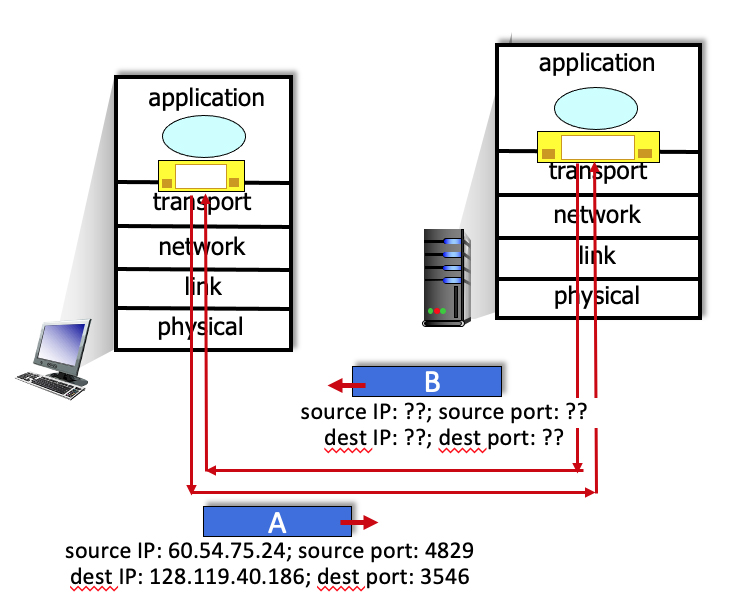
\includegraphics[width=0.5\textwidth]{img/3.3.9.jpg}
        \label{fig:UDP}
    \end{figure}
    \begin{itemize}
        \item The source port number of the UDP segment (B) sent in reply is: \textbf{3546}
        \item The source IP address of the IP datagram containing the UDP segment (B) sent in reply is: \textbf{128.119.40.186}
        \item The destination port number of the UDP segment (B) sent in reply  is: \textbf{4829}
        \item The destination IP address of the IP datagram containing the UDP segment (B) sent in reply is: \textbf{60.54.75.24}
    \end{itemize}

\newpage
\subsection*{Principles of Reliable Data Transfer}
    \subsubsection*{Reliable data transfer protocol mechanisms}
    \noindent Consider the purpose/goals/use of different reliable data transfer protocol mechanism. For the given
    purpose/goal/use this is the RDT mechanism that is used to implement the given purpose/goal/use
    \begin{itemize}
        \item[NAK] Lets the sender know that a packet was NOT received correctly at the receiver
        \item[Checksum] Used by the sender or receiver to detect bits flipped during a packet's transmission
        \item[Sequence numbers] Allows for duplicate detection at receiver
        \item[ACK] Lets the sender know that a packet was received correctly at the receiver  
        \item[Retransmission] Allows the receiver to eventually receive a packet that was corrupted or lost in an
        earlier transmission
    \end{itemize}

    \subsubsection*{Cumulative ACK}
    \noindent What is meant by cumulative acknowledgment, ACK(\textit{n})?
    A cumulative ACK(\textit{n}) acks all packets with a sequence number up to and including \textit{n} as being received

    \subsubsection*{Stop-and-wait: channel utilization}
    \noindent Suppose a packet is 10k bits long, the channel transmission rate connecting a sender and receiver is
    10 Mbps, and the round-trip propagation delay is 10 ms. What is the maximum channel utilization of a stop-and-wait
    protocol for this channel?
    \[U_{sender}=\frac{L/R}{RTT+L/R}=\frac{10,000/10,000,000}{0.01+10,000/10,000,000}=0.09\approx0.1\]
    where
    \begin{itemize}
        \item[L] packet size 
        \item[R] transmission rate
        \item[RTT]  Round-trip propagation
    \end{itemize}

    \newpage
    \subsubsection*{Channel utilization with pipelining}
    \noindent Suppose a packet is 10K bits long, the channel transmission rate connecting a sender and receiver is
    10 Mbps, and the round-trip propagation delay is 10 ms. What is the channel utilization if a pipelined protocol
    with an arbitrarily high level of pipelining for this channel?
    \[U_{sender}=\frac{N*L/R}{RTT+L/R}\]
    where
    \begin{itemize}
        \item[L] packet size 
        \item[R] transmission rate
        \item[RTT]  Round-trip propagation
        \item[N] packet pipelining increased utilization 
    \end{itemize}

    \subsubsection*{Channel utilization with pipelining (more)}
    \noindent Suppose a packet is 10K bits long, the channel transmission rate connecting a sender and receiver is
    10 Mbps, and the round-trip propagation delay is 10 ms. How many packets can the sender transmit before it starts
    receiving acknowledgment back?
    The answer is 10 packets

    \subsubsection*{Pipelining}
    \noindent The next statements are true about pipelining:
    \begin{itemize}
        \item A pipelined sender can have trasmitted multiple packets for which the sender has yet to receive an ACK from the
        receiver
        \item With a pipelined sender, there may be transmitted packet "in flight" - propagating through the channel - packets
        that the sender has sent but that the receiver has not yet received
    \end{itemize}

    \subsubsection*{Packet buffering in Go-Back-N}
    \noindent What are some reasons for discarding received-but-out-of-sequence packets at the receiver in GBN?
    \begin{itemize}
        \item The sender will resedn that packet in any case
        \item The implementation at the receiver is simpler
    \end{itemize}

    \subsubsection*{Packet buffering in Go-Back-N (more)}
    \noindent What are some reasons for \textit{not} discarding received-but-out-of-sequence packets at the receiver in GBN?
    \begin{itemize}
        \item Even though that packet will be retransmitted, its next retransmission could be corrupted, so don't discard
        a perfectly well-received packet
    \end{itemize}

    \subsubsection*{Receiver operation in Selective Repeat}
    \noindent In the SR receiver window (see diagram below), why haven't the red packets been delivered yet?
    \begin{figure}[H]
        \centering
        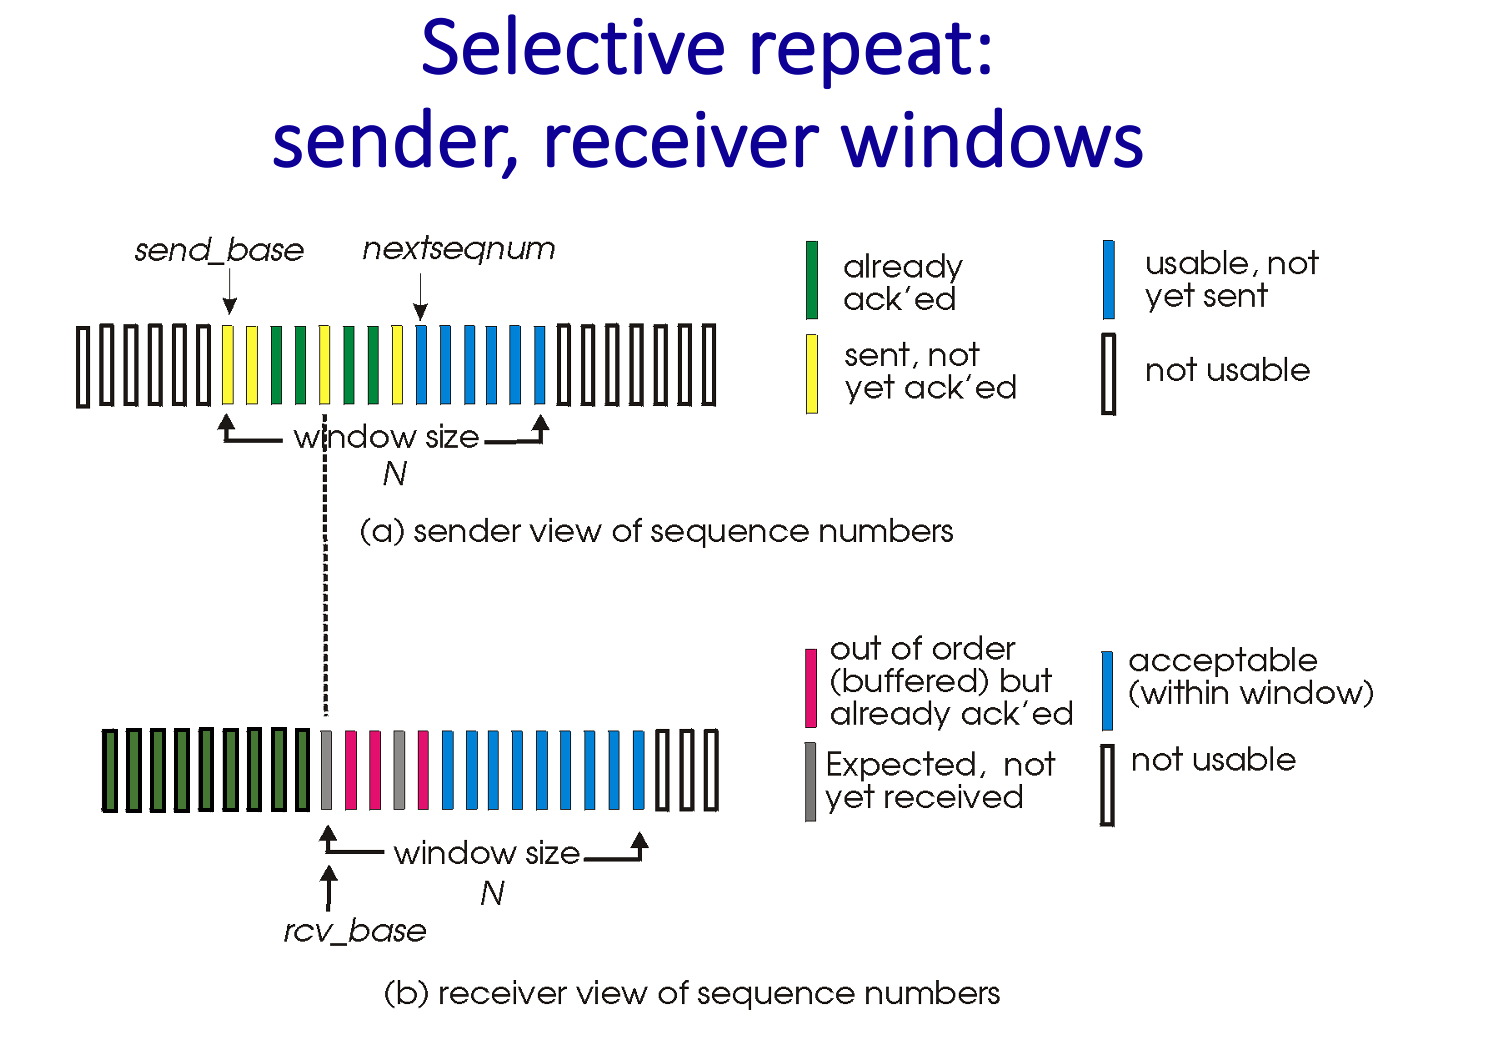
\includegraphics[width=0.5\textwidth]{img/3.4.13.jpg}
    \end{figure}
    There is a packet with a lower sequence number than any of the red packets that has yet to be received, so in-order dalivery
    of data in the red packets up to the application layer is not possible

    \subsubsection*{Receiver operation in Selective Repeat (more)}
    \noindent In SR, why does the receiver have to acknowledge packets with sequence numbers that are less than those in its 
    window, which starts at \textit{rcv-base}
    \begin{figure}[H]
        \centering
        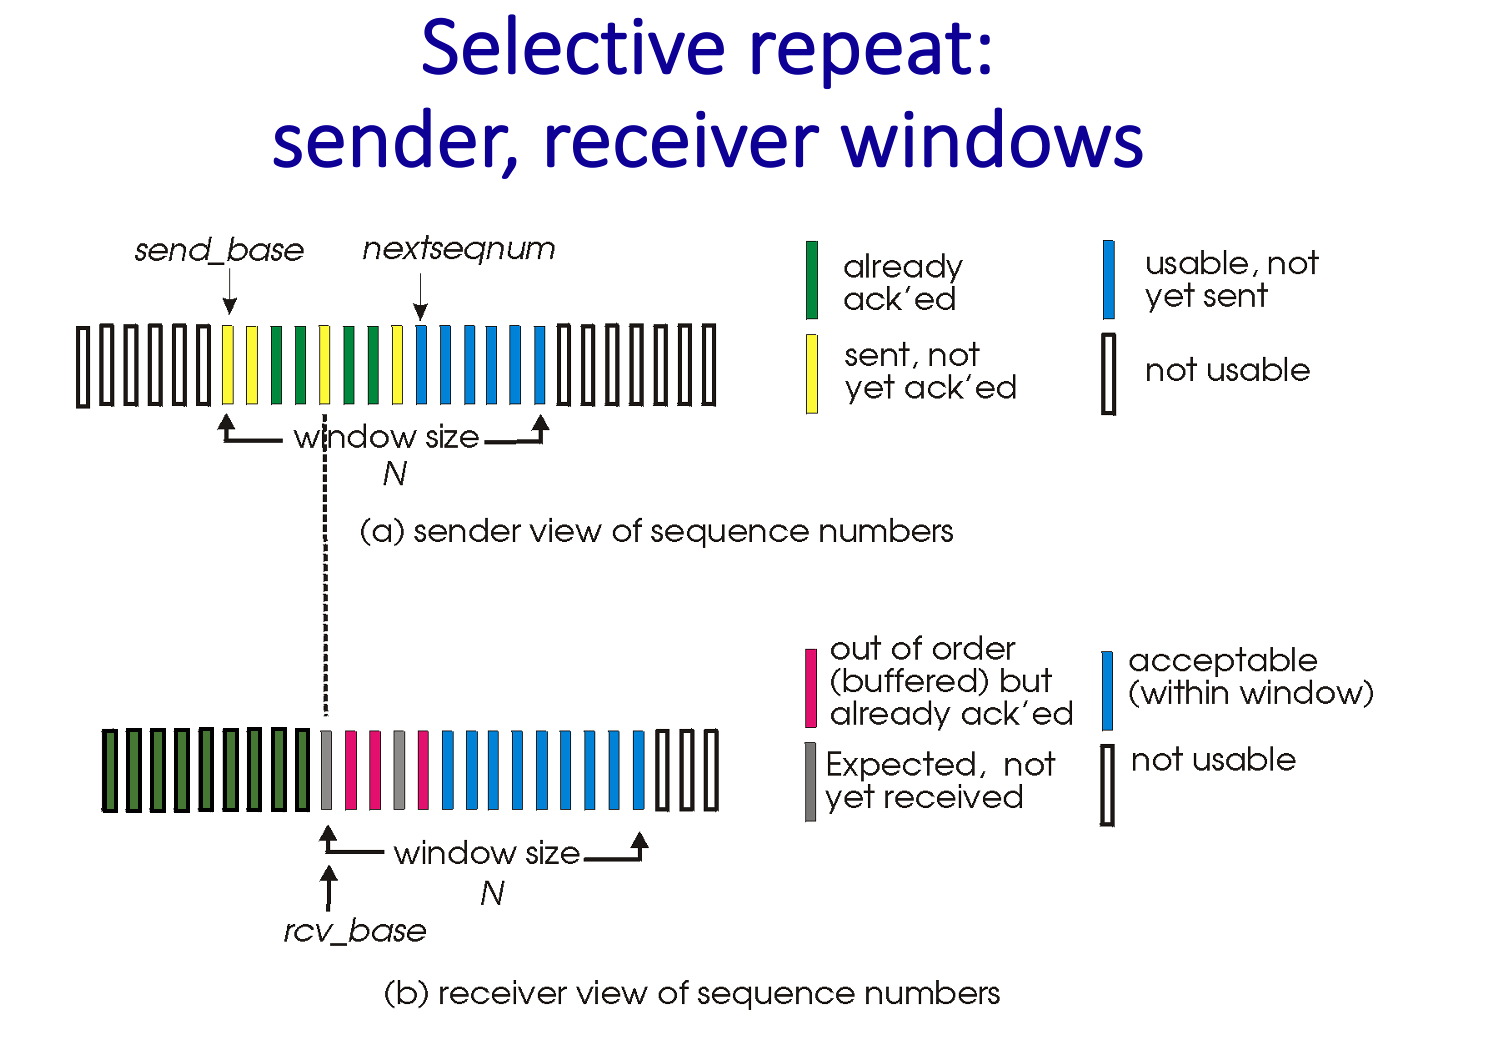
\includegraphics[width=0.5\textwidth]{img/3.4.13.jpg}
    \end{figure}
    Because the sender may not have received an ACK for that packet yet.

\newpage
\subsection*{Connection-oriented Transport: TCP}
    \subsubsection*{TCP reliability semantics}
    \noindent \textbf{[FALSE]} On the sending side, the TCP sender will take each application-layer chunk of data written into a TCP socket and send it 
    in a distinct TCP segment. And on the receiving side, TCP will deliver a segment's payload into the appropiate socket, preserving
    the application-defined message boundary.

    \subsubsection*{TCP segment format}
    \begin{description}
        \item[Socket port number] This field contains the port number associated with the sending socket for this TCP segment.
        \item[Data (\textit{or payload})] This field contains application data that was written into a socket by the sender of this TCP segment.
        \item[Sequence number] This field contains the index in the sender-to-receiver byte stream of the first byte of that data in the payload carried in this segment.
        \item[ACK number field] This field contains the index in the byte stream of the next in-order byte expected at the receiver.
        \item[ACK bit] If set, this segment cumulatively ACKs in the byte all data bytes up to, but not including, the byte index in the ACK value field of this segment.
        \item[Receiver advertised window] This field contains the number of available bytes in the TCP receiver's buffer.
        \item[Checksum] This field contains the Internet checksum of the TCP segment and selected fields in the IP datagram header.
        \item[Header length field] This field contains the number of bytes in the TCP header.        
    \end{description}

    \subsubsection*{TCP sequence numbers and ACKs (1)}
    \noindent Consider the TCP Telnet scenario below. Why is it that the receiver sends an ACK that is one larger than the sequence number in the received datagram?
    \begin{figure}[H]
        \centering
        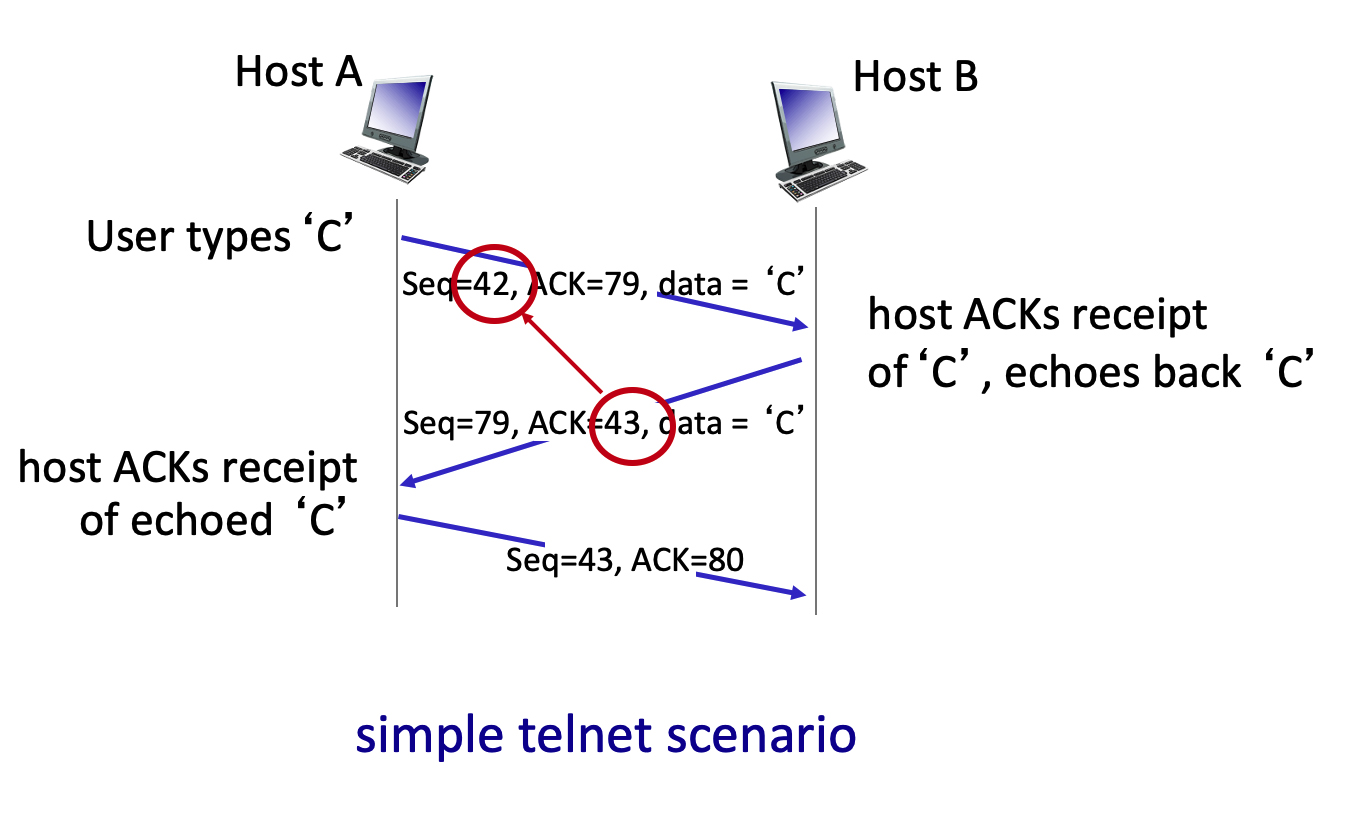
\includegraphics[width=0.5\textwidth]{img/3.5.3.jpg}
    \end{figure}
    \noindent Because the send-to receiver segment carries only one byte of data, and after that segment is received, the next expected byte of data is just the next
    byte (\textit{i.e., has an index that is one larger}) in the data stream.

    \subsubsection*{TCP sequence numbers and ACKs (2)}
    \noindent Suppose that as shown in the figure below, a TCP sender is sending segments with 100 bytes of payload. The TCP sender sends five segments with sequence
    numbers 100, 200, 300, 400, and 500. Suppose that the segment with sequence number 300 is lost. The TCP receiver will buffer correctly-received but not-yet-in-order
    segments for later delivery to the application layer (\textit{once missing segments are later received})
    \begin{figure}[H]
        \centering
        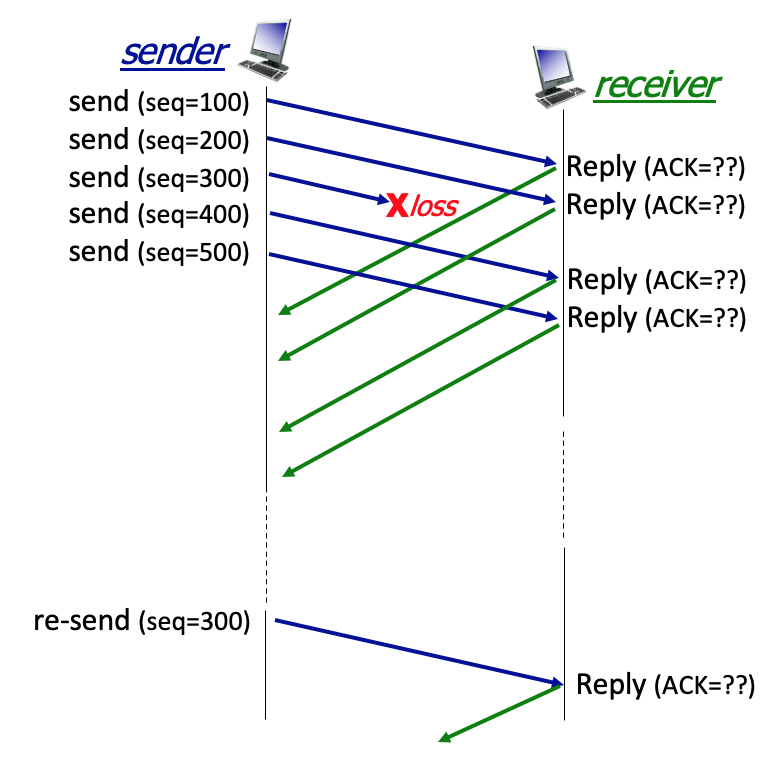
\includegraphics[width=0.5\textwidth]{img/3.5.4.jpg}
    \end{figure}
    \begin{itemize}
        \item After receiving segment 100, the receiver responds with an ACK with value \textbf{200}.
        \item After receiving segment 200, the receiver responds with an ACK with value \textbf{300}.
        \item After receiving segment 500, the receiver responds with an ACK with value \textbf{300, a duplicate ACK}.
        \item After receiving the retransmitted segment 300, the receiver responds with an ACK with value \textbf{600}.
        \item The TCP receiver does not respond in the example, with an ACK with value \textbf{400}.
    \end{itemize}

    \subsubsection*{TCP RTT Estimation: EWMA}
    \noindent Consider TCP use of an exponentially weighted moving average (\textit{EWMA}) to compute the nth value of the estimated RTT:
    $$ EstimatedRTT_n ) (1-a)*EstimatedRTT_{n-1} + a*SampleRTT_n $$
    \noindent \textbf{[FALSE]} with this EWMA algorithm the alue of \(EstimatedRTT_n\) has no dependence on the earlier sample, \( SampleRTT_{n-1}\).

    \subsubsection*{TCP timer management}
    \noindent Consider the TCP Telnet below. What timer-related action does the sender take on the receipt of ACK 120?
    \begin{figure}[H]
        \centering
        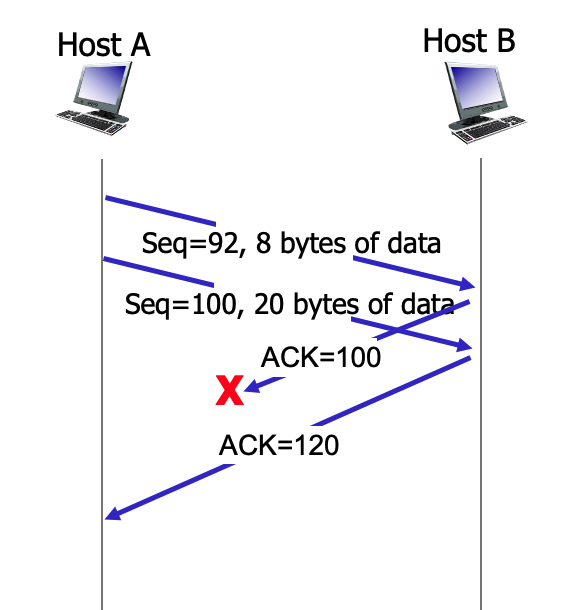
\includegraphics[width=0.5\textwidth]{img/3.5.6.jpg}
    \end{figure}
    \noindent Cancels any running timers.

    \subsubsection*{TCP Flow Control}
    \noindent With TCP's flow control mechanism, where the receiver tells the sender how much free buffer space it has (\textit{and the sender always limits the amount
    of outstanding, unACKed, in-flight to less than this amount}), it is not possible for the sender to send more that the receiver has room to buffer.

    \subsubsection*{TCP connection management}
    \begin{description}
        \item[SYN MESSAGE] A message from client to server initiating a connection request.
        \item[SYNACK MESSAGE] A message from server to client ACKing receipt of a SYN message and indicating the willingness of the server to establish a TCP connection with the client.
        \item[FIN MESSAGE] A message indicating that the sending side is initiating the protocol to terminate a connection.
        \item[FINBACK MESSGE] A message sent in response to a request to terminate a connection. ACKing that the side receiving this message is algo willing to terminate the connection.
        \item[RESET MESSAGE] A general purpose error message used during connection set up or tear down to let the other side know that an error has ocurred, and that the referenced connection
        should be shut down.     
    \end{description}

    \subsubsection*{TCP Fast Retransmit}
    \noindent Consider the TCPs Fast Retransmit optmization. Of course, the sender doesn't know for sure that the segment with sequence \#100 is actually lost (\textit{it can't see into the channel}).
    Can a sender get three duplicate ACKs for a segment that in fact has \textit{not} been lost? The following statements are true. Suppose a channel can lose, but will not corrupt, messages.
    \begin{itemize}
        \item If the channel can reorder messages, a triple duplicate ACK can occure even though a message is not lost; since it's possible that a message has just been reordered and has not
        yet arrived when the three ACKs were generated.
        \item If the channel cannot reorder messages, a triple duplicate ACK indicates to the sender that a segment loss has happened for sure. Actually (\textit{again assuming the channel cannot
        corrupt or reorder messages}), even a \textit{single} duplicate ACK would indicate that a segment loss has happend for sure.
    \end{itemize}

\subsection*{Principles of Congestion Control}
    \subsubsection*{Congestion control versus flow control}
    \noindent Between the next options a \textbf{a glass overflowing} and \textbf{a talking head} are concepts that need flow control. The others would suggest the need for congestion control
    \begin{itemize}
        \item A penguin crowd
        \item Car traffic
        \item A crowd of people
        \item A glass overflowing
        \item A talking head
    \end{itemize}

    \subsubsection*{Two congested senders}
    \noindent Consider the figure below, which shows the application-to-application throughput achieved when two senders are competing at a shared bottleneck link. Suppose that then the overall
    arrival rate, \( lambd_{in}\)(\textit{for each sender}) is closer to R/2, the throughput to the application layer (\textit{at each receiver}), \(lambda_{out}\), is equal to \(0.8*lambda_{in}\).
    \begin{figure}[H]
        \centering
        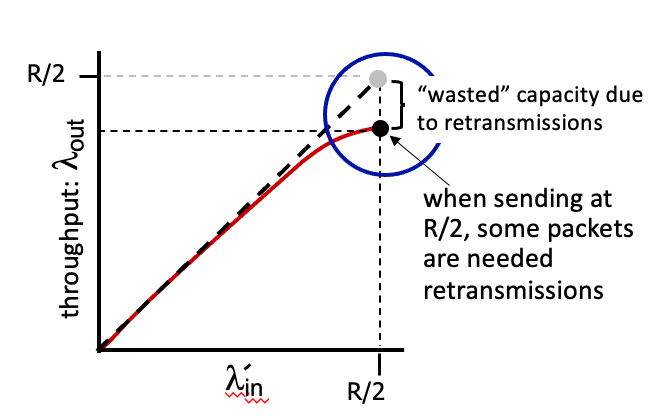
\includegraphics[width=0.5\textwidth]{img/3.6.2.jpg}
    \end{figure}
    \noindent What fraction of the packets transmitted at the sender are retransmissions? \textbf{0.20}

    \subsubsection*{Different approaches towards congestion control}
    \noindent Here are some options of how the sender detects congestion:
    \begin{description}
        \item[End-end] The sender infers segment loss from the absence of an ACK from the receiver.
        \item[Network-assisted] Bits are set at a congested router in a sender-to-receiver datagram, and bits are in the returned to the sender in a receiver-to-sender ACK, to indicate congestion to
        the sender.
        \item[Delay-based] The sender measure RTTs and uses the current RTT measurement in onfer the level of congestion.  
    \end{description}

\subsection*{TCP Congestion Control}
    \subsubsection*{TCPs AIMD algorithm}
    \noindent The following statements are true about TCP's Additive-increase-multiplicative-decrease (\textit{AIMD}) algorithm:
    \begin{itemize}
        \item AIMD cuts the congestion window size, cwnd, in half whenever loss is detected by a triple duplicate ACK.
        \item AIMD cuts the congestion window size, cwnd, i to 1 whenever a timeout occurs.
        \item AIMD is a end-end approach to congestion control
    \end{itemize}

    \subsubsection*{TCPs AIMD algorithm (2)}
    \noindent How is the sending rate typically regulated in a TCP implementation? By keeping a window size cwnd over the sequence number space, and making sure that no more than cwnd bytes of data
    are outstanding (\textit{i.e., unACKnowledged}). The size of cwnd ir regulated by AIMD.

    \subsubsection*{TCPs Slowstart algorithm}
    \noindent Consider the transport-layer flows interacting at a congested link. In the face of such congestion, what happens at this link to a transport-layer flow that does not cut back o its sending rate?
    Nothing different from the other flows crossing the congested link.